\problemname{Talis' Fireball}

The battle had been raging for many rounds and your party is tired. Things are looking dark, until the wizard Talis realizes he has a 3rd level spell slot left. 
That's enough for a Fireball! But while Talis is searching for his scroll, he drops his glasses. They fall to the ground and shatter into pieces. Now you all need to work together to find out how many people Talis can hit.
\\
\\
Your team will shout the amount of enemies and their coordinates to you. Then they will also shout their location, just so Talis doesn't hit them. Now it is up to you to find out how many enemies Talis can hit with one fireball. Once you tell him the max amount of enemies he can hit, Talis will use his wizard energy to feel where the fireball should hit on the battlefield.
\\
\\
Talis, having no situational awareness, states multiple rules for where he is willing to place the fireball and how big it is. While the rest of your party holds the enemies at bay.
\\
\\
All enemies and allies will be placed on a grid, like shown in the diagram below. The fireball must be placed in the middle of a square. An enemy is considered hit by a fireball if the middle of the square is within the circle the fireball creates. The radius of this circle is $2.5 m$. On the diagram below, the red squares represent the area the fireball hits. The fireball cannot hit any ally, or Talis will refuse to throw it. Additionally, the fighting have only spread out to an area of around $1200 m * 1200 m$, so that is where all enemies and allies will be.


\begin{center}
  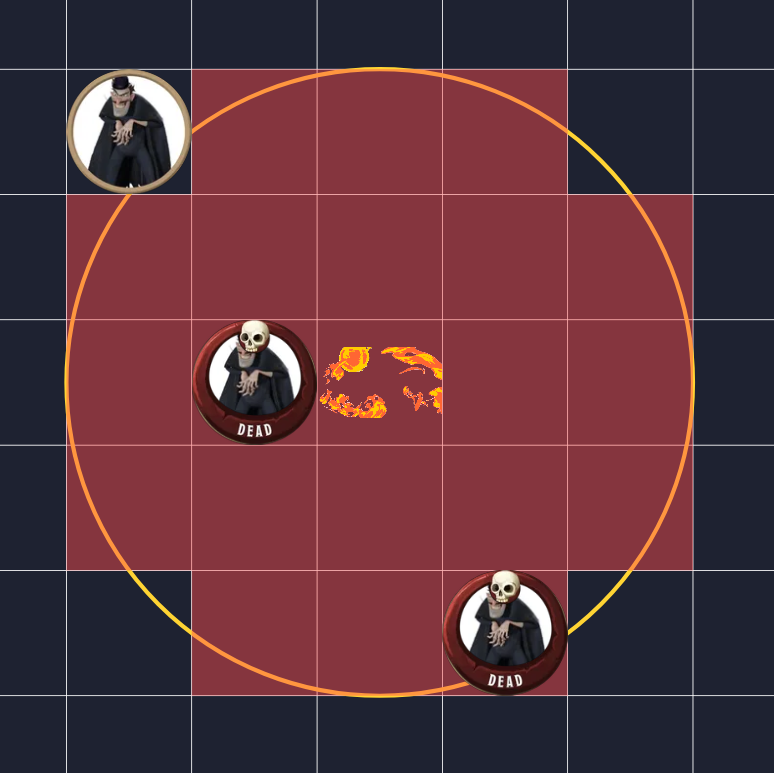
\includegraphics[width=0.5\textwidth]{Example.png}
\end{center}

\section*{Input}

The input consist of 4 lines. 
First line containing the number e of enemies on the battlefield $0 \leq e \leq 100000$\\
Then follows e lines of (x, y) coordinates for the enemies $0 \leq x, y \leq 1200$ \\
Then a line containing the number f of party-members on the battlefield $0 \leq f \leq 100000$ \\
Then follows f lines of (x, y) coordinates for the party-members $0 \leq x, y \leq 1200$ 

\section*{Output}

Output a single integer giving the maximum number of enemies a single fireball can hit at once, without hitting any party-members.
